\documentclass[11pt,a4paper]{article}

\usepackage[margin=2.2cm]{geometry}
\usepackage[utf8]{inputenc}
\usepackage{amsmath,amssymb}
\usepackage{graphicx}
\usepackage{subcaption}
\usepackage{listings}
\usepackage{xcolor}
\usepackage{hyperref}
\usepackage{float}
\usepackage{tikz}
\usepackage{booktabs}
\usepackage{enumitem}
\usepackage{caption}

\usetikzlibrary{shapes,arrows,positioning,calc,decorations.pathreplacing}

\graphicspath{{../}}

% Reasonable spacing
\setlength{\parskip}{0.5em}
\setlength{\parindent}{0pt}
\setlist{itemsep=2pt, topsep=4pt}

% Code style
\definecolor{codegreen}{rgb}{0,0.6,0}
\definecolor{backcolour}{rgb}{0.96,0.96,0.93}
\lstdefinestyle{matlab}{
    backgroundcolor=\color{backcolour},
    commentstyle=\color{codegreen},
    keywordstyle=\color{blue}\bfseries,
    basicstyle=\ttfamily\small,
    breaklines=true,
    numbers=left,
    numberstyle=\tiny\color{gray},
    numbersep=5pt,
    frame=single,
    language=Matlab,
}
\lstset{style=matlab}

% TikZ styles
\tikzstyle{vertex} = [circle, draw, fill=orange!80, minimum size=0.8cm, font=\small\bfseries]
\tikzstyle{landmark} = [circle, draw, fill=green!60, minimum size=0.8cm, font=\small\bfseries]
\tikzstyle{factor} = [rectangle, fill=black, minimum size=0.22cm]

\title{\textbf{COMP0222 Coursework 01: Graph-based Optimisation and SLAM}}
\author{Group XX\\Department of Computer Science, University College London}
\date{\today}

\begin{document}
\maketitle

%==============================================================================
\section{Question 1: GPS-only Localization [31 marks]}
%==============================================================================

\subsection{1a. Factor Graph Structure [15 marks]}

The GPS-only localization problem is formulated as a factor graph with vertices representing unknown states and edges (factors) representing probabilistic constraints.

\subsubsection*{Vertices}

\textbf{Platform State Vertex} ($\mathbf{x}_k$): Represents the vehicle state at timestep $k$:
\begin{equation}
\mathbf{x}_k = \begin{bmatrix} x_k \\ y_k \\ \psi_k \end{bmatrix}
\end{equation}
where $(x_k, y_k)$ is position and $\psi_k$ is heading angle.

\textbf{Addition Operator:} $\mathbf{x} \oplus \delta\mathbf{x} = \mathbf{x} + \delta\mathbf{x}$ with heading wrapped to $[-\pi, \pi]$.

\subsubsection*{Edges (Factors)}

\begin{enumerate}
\item \textbf{Initial Prior Edge} (Unary): Connects to $\mathbf{x}_0$. Measurement: initial state $\mathbf{z}_0$. Error: $\mathbf{e} = \mathbf{x}_0 - \mathbf{z}_0$. Information: $\boldsymbol{\Omega}_0 = \mathbf{P}_0^{-1}$.

\item \textbf{Platform Prediction Edge} (Binary): Connects $\mathbf{x}_k$ to $\mathbf{x}_{k+1}$. Uses the process model (Eq.~3, Appendix A.2):
\begin{equation}
\mathbf{x}_{k+1} = \mathbf{x}_k + \mathbf{M}(\psi_k)\mathbf{u}_{k+1}, \quad \text{where } \mathbf{M} = \Delta T \begin{bmatrix} \cos\psi_k & -\sin\psi_k & 0 \\ \sin\psi_k & \cos\psi_k & 0 \\ 0 & 0 & 1 \end{bmatrix}
\end{equation}
Measurement: odometry $\mathbf{u}_{k+1} = [s_{k+1}, 0, \dot{\psi}_{k+1}]^T$. Information: $\boldsymbol{\Omega}_Q = \mathbf{Q}^{-1}$.

\item \textbf{GPS Measurement Edge} (Unary): Connects to $\mathbf{x}_k$. Model (Appendix A.3):
\begin{equation}
\mathbf{z}^G_k = \begin{bmatrix} x_k \\ y_k \end{bmatrix} + \mathbf{w}^G_k
\end{equation}
Error: $\mathbf{e} = \mathbf{z}^G - [x_k, y_k]^T$. Information: $\boldsymbol{\Omega}_R = (\mathbf{R}^G)^{-1}$.
\end{enumerate}

\begin{figure}[H]
\centering
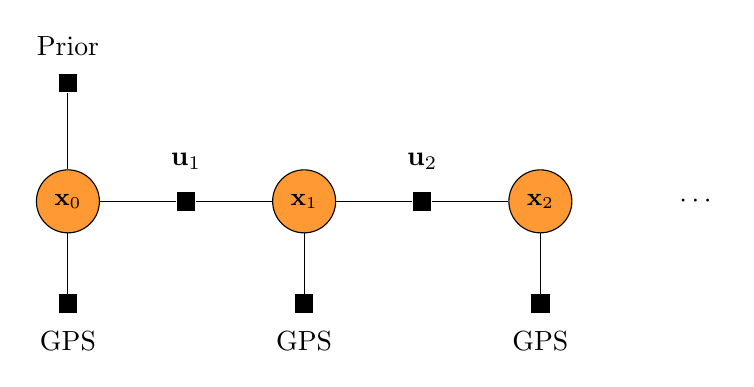
\begin{tikzpicture}[scale=1.0]
    \node[vertex] (x0) at (0,0) {$\mathbf{x}_0$};
    \node[vertex] (x1) at (3,0) {$\mathbf{x}_1$};
    \node[vertex] (x2) at (6,0) {$\mathbf{x}_2$};
    \node at (8,0) {$\cdots$};

    \node[factor] (prior) at (0,1.5) {};
    \draw (prior) -- (x0);
    \node[above=0.1cm of prior] {Prior};

    \node[factor] (f01) at (1.5,0) {};
    \node[factor] (f12) at (4.5,0) {};
    \draw (x0) -- (f01) -- (x1) -- (f12) -- (x2);
    \node[above=0.15cm of f01] {$\mathbf{u}_1$};
    \node[above=0.15cm of f12] {$\mathbf{u}_2$};

    \node[factor] (g0) at (0,-1.3) {};
    \node[factor] (g1) at (3,-1.3) {};
    \node[factor] (g2) at (6,-1.3) {};
    \draw (g0) -- (x0); \draw (g1) -- (x1); \draw (g2) -- (x2);
    \node[below=0.1cm of g0] {GPS};
    \node[below=0.1cm of g1] {GPS};
    \node[below=0.1cm of g2] {GPS};
\end{tikzpicture}
\caption{Factor graph for GPS-only localization. Orange circles: platform vertices. Black squares: factors.}
\end{figure}

\textbf{Optimization Objective:}
\begin{equation}
\mathbf{x}^* = \arg\min_{\mathbf{x}_{0:K}} \sum_i \mathbf{e}_i^T \boldsymbol{\Omega}_i \mathbf{e}_i
\end{equation}

\subsection{1b. PlatformPredictionEdge Implementation [9 marks]}

\subsubsection*{initialEstimate()}
Predicts $\mathbf{x}_{k+1}$ from $\mathbf{x}_k$ using the process model:

\begin{lstlisting}
function initialEstimate(obj)
    x_k = obj.edgeVertices{1}.x;
    theta = x_k(3);
    u = obj.z;  % odometry measurement [vx; vy; omega]

    % Rotation matrix M (Eq. 4, Appendix A.2)
    M = obj.dT * [cos(theta), -sin(theta), 0;
                  sin(theta),  cos(theta), 0;
                  0,           0,          1];

    % Predict next state: x_{k+1} = x_k + M * u
    x_kp1 = x_k + M * u;
    x_kp1(3) = g2o.stuff.normalize_theta(x_kp1(3));
    obj.edgeVertices{2}.setEstimate(x_kp1);
end
\end{lstlisting}

\subsubsection*{computeError()}
Computes error as $\mathbf{e} = \mathbf{M}^{-1}(\mathbf{x}_{k+1} - \mathbf{x}_k) - \mathbf{z}$:

\begin{lstlisting}
function computeError(obj)
    x_k = obj.edgeVertices{1}.x;
    x_kp1 = obj.edgeVertices{2}.x;
    theta = x_k(3);
    dx = x_kp1 - x_k;

    % Inverse of M: inv(M) = (1/dT) * R(-theta)
    c = cos(theta); s = sin(theta);
    invM = (1/obj.dT) * [c, s, 0; -s, c, 0; 0, 0, 1];

    obj.errorZ = invM * dx - obj.z;
    obj.errorZ(3) = g2o.stuff.normalize_theta(obj.errorZ(3));
end
\end{lstlisting}

\subsubsection*{linearizeOplus()}
Computes Jacobians $\mathbf{J}_1 = \partial\mathbf{e}/\partial\mathbf{x}_k$ and $\mathbf{J}_2 = \partial\mathbf{e}/\partial\mathbf{x}_{k+1}$:

\begin{lstlisting}
function linearizeOplus(obj)
    x_k = obj.edgeVertices{1}.x;
    x_kp1 = obj.edgeVertices{2}.x;
    theta = x_k(3);
    dx = x_kp1 - x_k;
    c = cos(theta); s = sin(theta);
    invDT = 1/obj.dT;

    % J{2} = de/dx_{k+1} = inv(M)
    obj.J{2} = invDT * [c, s, 0; -s, c, 0; 0, 0, 1];

    % J{1} = de/dx_k (includes derivative of inv(M) w.r.t. theta)
    obj.J{1} = invDT * [-c, -s, -s*dx(1)+c*dx(2);
                         s, -c, -c*dx(1)-s*dx(2);
                         0,  0, -1];
end
\end{lstlisting}

\textbf{Results:} Figure~\ref{fig:q1b_errors} shows the position errors from running \texttt{cw1.q1\_b}. The errors (yellow) remain within the $\pm 2\sigma$ bounds (red dashed), confirming filter consistency.

\begin{figure}[H]
\centering
\begin{subfigure}[b]{\textwidth}
    \centering
    \includegraphics[width=0.85\textwidth]{q1_b.png}
    \caption{$x$ position error}
\end{subfigure}
\vspace{0.3em}
\begin{subfigure}[b]{\textwidth}
    \centering
    \includegraphics[width=0.85\textwidth]{q1_b2.png}
    \caption{$y$ position error}
\end{subfigure}
\caption{Q1b: Position errors with $\pm 2\sigma$ bounds (red dashed). Errors remain bounded, demonstrating consistency of the factor graph localization system.}
\label{fig:q1b_errors}
\end{figure}

\subsection{1c. Graph Optimization Analysis [7 marks]}

Running \texttt{cw1.q1\_c} produces the plots in Figure~\ref{fig:q1c_results}.

\textbf{Observed Trends:}
\begin{itemize}
\item The $\chi^2$ values increase monotonically over time in a staircase pattern, reaching approximately 14 over 850 time steps. Each step corresponds to a new GPS measurement being added to the graph.
\item The optimization time shows a general upward trend with intermittent spikes, indicating that the optimizer occasionally requires more iterations as the graph grows.
\end{itemize}

\textbf{Relationship:} Both metrics are driven by the growing graph size. Each timestep adds new vertices and edges, causing:
\begin{itemize}
\item More error terms contribute to $\chi^2 = \sum_i \mathbf{e}_i^T \boldsymbol{\Omega}_i \mathbf{e}_i$, so the total cost increases
\item The Hessian matrix grows, increasing the computational cost of the sparse linear solve
\end{itemize}

\textbf{Underlying Cause:} The graph grows unboundedly---no pruning or marginalization is performed, so both the cost function value and the time to optimize it increase with each new measurement.

\begin{figure}[H]
\centering
\begin{subfigure}[b]{\textwidth}
    \centering
    \includegraphics[width=0.85\textwidth]{q1_c.png}
    \caption{$\chi^2$ values vs.\ time step}
\end{subfigure}
\vspace{0.3em}
\begin{subfigure}[b]{\textwidth}
    \centering
    \includegraphics[width=0.85\textwidth]{q1_c2.png}
    \caption{Optimization time vs.\ time step}
\end{subfigure}
\caption{Q1c: $\chi^2$ and optimization time both increase over time due to unbounded graph growth.}
\label{fig:q1c_results}
\end{figure}

%==============================================================================
\section{Question 2: Full SLAM Implementation [36 marks]}
%==============================================================================

\subsection{2a. Factor Graph Structure for Full SLAM [9 marks]}

\subsubsection*{Additional Vertex}

\textbf{Landmark State Vertex} ($\mathbf{m}_i$): 2D position of the $i$-th landmark:
\begin{equation}
\mathbf{m}_i = \begin{bmatrix} x_i \\ y_i \end{bmatrix}
\end{equation}
\textbf{Addition Operator:} $\mathbf{m} \oplus \delta\mathbf{m} = \mathbf{m} + \delta\mathbf{m}$ (standard Euclidean).

\subsubsection*{Additional Edge}

\textbf{Landmark Range-Bearing Edge} (Binary): Connects platform $\mathbf{x}_k$ to landmark $\mathbf{m}_i$. Model (Appendix A.4):
\begin{equation}
\mathbf{z}^L = \begin{bmatrix} r \\ \beta \end{bmatrix}, \quad r = \sqrt{(x_i-x_k)^2 + (y_i-y_k)^2}, \quad \beta = \text{atan2}(y_i-y_k, x_i-x_k) - \psi_k
\end{equation}

\begin{figure}[H]
\centering
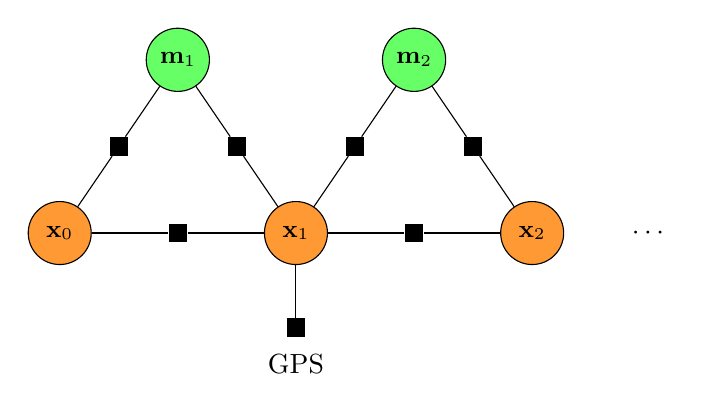
\begin{tikzpicture}[scale=1.0]
    \node[landmark] (m1) at (1.5,2.2) {$\mathbf{m}_1$};
    \node[landmark] (m2) at (4.5,2.2) {$\mathbf{m}_2$};

    \node[vertex] (x0) at (0,0) {$\mathbf{x}_0$};
    \node[vertex] (x1) at (3,0) {$\mathbf{x}_1$};
    \node[vertex] (x2) at (6,0) {$\mathbf{x}_2$};
    \node at (7.5,0) {$\cdots$};

    \node[factor] (f01) at (1.5,0) {};
    \node[factor] (f12) at (4.5,0) {};
    \draw (x0) -- (f01) -- (x1) -- (f12) -- (x2);

    \node[factor] (o1) at (0.75,1.1) {};
    \node[factor] (o2) at (2.25,1.1) {};
    \node[factor] (o3) at (3.75,1.1) {};
    \node[factor] (o4) at (5.25,1.1) {};
    \draw (x0) -- (o1) -- (m1); \draw (x1) -- (o2) -- (m1);
    \draw (x1) -- (o3) -- (m2); \draw (x2) -- (o4) -- (m2);

    \node[factor] (gps) at (3,-1.2) {};
    \draw (gps) -- (x1);
    \node[below=0.1cm of gps] {GPS};
\end{tikzpicture}
\caption{Full SLAM factor graph. Green: landmark vertices. Orange: platform vertices.}
\end{figure}

\subsection{2b. LandmarkRangeBearingEdge Implementation [14 marks]}

\subsubsection*{initialEstimate()}
Initializes landmark position using inverse observation model:

\begin{lstlisting}
function initialEstimate(obj)
    x = obj.edgeVertices{1}.x;  % platform state [px; py; theta]
    r = obj.z(1);               % range measurement
    beta = obj.z(2);            % bearing measurement

    % World-frame angle to landmark
    phi = x(3) + beta;

    % Inverse observation model
    lx = x(1) + r * cos(phi);
    ly = x(2) + r * sin(phi);
    obj.edgeVertices{2}.setEstimate([lx; ly]);
end
\end{lstlisting}

\subsubsection*{computeError()}
Computes error $\mathbf{e} = \mathbf{z} - \mathbf{h}(\mathbf{x}, \mathbf{m})$:

\begin{lstlisting}
function computeError(obj)
    x = obj.edgeVertices{1}.x;  % platform [px; py; theta]
    l = obj.edgeVertices{2}.x;  % landmark [lx; ly]

    dx = l(1) - x(1);
    dy = l(2) - x(2);

    r_pred = sqrt(dx^2 + dy^2);
    beta_pred = atan2(dy, dx) - x(3);

    obj.errorZ = obj.z - [r_pred; beta_pred];
    obj.errorZ(2) = g2o.stuff.normalize_theta(obj.errorZ(2));
end
\end{lstlisting}

\subsubsection*{linearizeOplus()}
Computes Jacobians w.r.t. platform and landmark:

\begin{lstlisting}
function linearizeOplus(obj)
    x = obj.edgeVertices{1}.x;
    l = obj.edgeVertices{2}.x;
    dx = l(1) - x(1);  dy = l(2) - x(2);
    r2 = dx^2 + dy^2;  r = sqrt(r2);
    if r < 1e-6, r = 1e-6; r2 = r^2; end

    % dh/dx (platform Jacobian)
    dh_dx = [-dx/r, -dy/r, 0; dy/r2, -dx/r2, -1];

    % dh/dl (landmark Jacobian)
    dh_dl = [dx/r, dy/r; -dy/r2, dx/r2];

    % e = z - h, so de/d(.) = -dh/d(.)
    obj.J{1} = -dh_dx;
    obj.J{2} = -dh_dl;
end
\end{lstlisting}

\textbf{Validation:} Figure~\ref{fig:q2b_map} shows the SLAM map from \texttt{cw1.q2\_b}. With noise disabled, EKF and G2O produce nearly identical estimates, confirming correct implementation.

\begin{figure}[H]
\centering
\includegraphics[width=0.75\textwidth]{q2_bmain.png}
\caption{Q2b: SLAM map with EKF (gray) and G2O (green). Both estimators produce matching results with noise disabled, validating the \texttt{LandmarkRangeBearingEdge} implementation.}
\label{fig:q2b_map}
\end{figure}

\subsubsection*{2b.ii Performance Analysis [7 marks]}

Figure~\ref{fig:q2b_perf} shows the $\chi^2$ and optimization time for the full SLAM system. Compared to Q1c (GPS-only, $\chi^2 \approx 14$ over 850 steps), the full SLAM system reaches $\chi^2 \approx 2100$ over 140 steps---growth is significantly faster because:
\begin{itemize}
\item Landmark vertices increase the graph size
\item Multiple observations per landmark add many edges at each time step
\item The graph structure becomes denser with landmark--platform cross-connections
\end{itemize}

The optimization time also shows a more pronounced increase, with spikes reaching up to 20 seconds, compared to the sub-second times in Q1c. This confirms that the computational cost scales with the number of edges and vertices in the graph.

\begin{figure}[H]
\centering
\begin{subfigure}[b]{\textwidth}
    \centering
    \includegraphics[width=0.85\textwidth]{q2_b5.png}
    \caption{$\chi^2$ values vs.\ time step}
\end{subfigure}
\vspace{0.3em}
\begin{subfigure}[b]{\textwidth}
    \centering
    \includegraphics[width=0.85\textwidth]{q2_b6.png}
    \caption{Optimization time vs.\ time step}
\end{subfigure}
\caption{Q2b: $\chi^2$ and optimization time for full SLAM. Both grow significantly faster than the GPS-only case (Q1c) due to landmark observation edges.}
\label{fig:q2b_perf}
\end{figure}

\subsection{2c. Large Scenario Analysis [13 marks]}

\subsubsection*{2c.i Consistency Analysis [5 marks]}

Figure~\ref{fig:q2c_map} shows the large scenario comparison. The EKF is clearly inconsistent while G2O remains consistent.

\begin{figure}[H]
\centering
\includegraphics[width=0.78\textwidth]{q2_cmain.png}
\caption{Q2c: Large scenario. EKF (gray) produces small, displaced ellipses that fail to contain true positions. G2O (green) produces appropriately sized ellipses that bound the true landmarks (crosses).}
\label{fig:q2c_map}
\end{figure}

\textbf{Evidence EKF is inconsistent} (see also Figure~\ref{fig:q2c_ekf_errors}):
\begin{itemize}
\item EKF covariance ellipses (gray) are small and displaced from true landmark positions
\item The EKF error plots show the position error reaching $-7$\,m ($x$) and $-10$\,m ($y$) while the $2\sigma$ bounds remain at approximately $\pm 1$\,m---the filter is severely overconfident
\item The heading error also significantly exceeds its $2\sigma$ bounds
\end{itemize}

\textbf{Evidence G2O is consistent} (see also Figure~\ref{fig:q2c_g2o_errors}):
\begin{itemize}
\item G2O covariance ellipses (green) properly bound true positions
\item Position and heading errors remain within $\pm 2\sigma$ bounds throughout the run
\end{itemize}

\begin{figure}[H]
\centering
\begin{subfigure}[b]{\textwidth}
    \centering
    \includegraphics[width=0.85\textwidth]{q2_c1.png}
    \caption{G2O $x$ error}
\end{subfigure}
\vspace{0.2em}
\begin{subfigure}[b]{\textwidth}
    \centering
    \includegraphics[width=0.85\textwidth]{q2_c2.png}
    \caption{G2O $y$ error}
\end{subfigure}
\vspace{0.2em}
\begin{subfigure}[b]{\textwidth}
    \centering
    \includegraphics[width=0.85\textwidth]{q2_c3.png}
    \caption{G2O $\theta$ error}
\end{subfigure}
\caption{Q2c: G2O error plots. All errors remain within $\pm 2\sigma$ bounds, confirming consistency.}
\label{fig:q2c_g2o_errors}
\end{figure}

\begin{figure}[H]
\centering
\begin{subfigure}[b]{\textwidth}
    \centering
    \includegraphics[width=0.85\textwidth]{q2_c4.png}
    \caption{EKF $x$ error---reaches $-7$\,m with $\pm 1$\,m bounds}
\end{subfigure}
\vspace{0.2em}
\begin{subfigure}[b]{\textwidth}
    \centering
    \includegraphics[width=0.85\textwidth]{q2_c5.png}
    \caption{EKF $y$ error---reaches $-10$\,m with $\pm 1$\,m bounds}
\end{subfigure}
\vspace{0.2em}
\begin{subfigure}[b]{\textwidth}
    \centering
    \includegraphics[width=0.85\textwidth]{q2_C6.png}
    \caption{EKF $\theta$ error---significantly exceeds bounds}
\end{subfigure}
\caption{Q2c: EKF error plots. All three state components significantly exceed the $\pm 2\sigma$ bounds, demonstrating severe inconsistency (overconfidence).}
\label{fig:q2c_ekf_errors}
\end{figure}

\subsubsection*{2c.ii Detection Range Impact [5 marks]}

The smaller detection range causes a significant divergence in performance because:
\begin{enumerate}
\item \textbf{Fewer observations per landmark:} With a smaller detection range, each landmark is observed fewer times and from fewer poses. This means larger state changes accumulate between observations, causing larger linearization errors in the EKF.
\item \textbf{Fewer loop closures:} The robot has less chance to re-observe previously seen landmarks, so accumulated drift cannot be corrected.
\item \textbf{EKF cannot revisit past estimates:} The EKF processes measurements sequentially and cannot update past states. G2O re-optimizes the entire trajectory globally when loop closures occur, correcting past errors that the EKF is unable to fix.
\end{enumerate}

\subsubsection*{2c.iii Detection Range Optimization [3 marks]}

Increasing \texttt{detectionRange} to approximately \textbf{25--30 meters} in \texttt{q2\_c/scenario.json} produces similar results for both algorithms.

\textbf{Why this works:}
\begin{itemize}
\item A larger detection range means more frequent landmark observations, keeping linearization errors small enough that the EKF's first-order approximation remains adequate
\item More overlapping observations provide better loop closure opportunities, reducing drift
\item With sufficiently frequent updates, the EKF and G2O operate in a similar regime where linearization errors are negligible
\end{itemize}

%==============================================================================
\section{Question 3: Graph Optimization Strategies [33 marks]}
%==============================================================================

\subsection{3a. Graph Pruning [14 marks]}

The pruning strategy limits each landmark to at most 4 observation edges, keeping the first and most recent observations.

\begin{figure}[H]
\centering
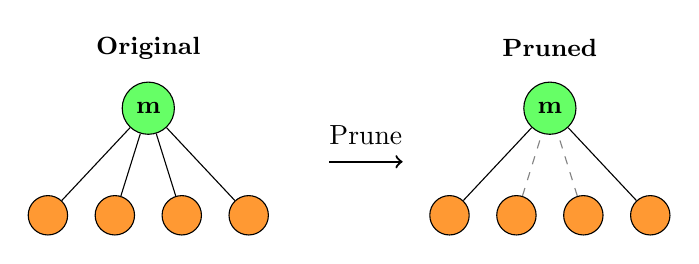
\begin{tikzpicture}[scale=0.85]
    \begin{scope}
        \node[font=\small\bfseries] at (1.5,2.5) {Original};
        \node[landmark, minimum size=0.6cm] (m) at (1.5,1.6) {$\mathbf{m}$};
        \node[vertex, minimum size=0.5cm] (a) at (0,0) {};
        \node[vertex, minimum size=0.5cm] (b) at (1,0) {};
        \node[vertex, minimum size=0.5cm] (c) at (2,0) {};
        \node[vertex, minimum size=0.5cm] (d) at (3,0) {};
        \draw (a)--(m); \draw (b)--(m); \draw (c)--(m); \draw (d)--(m);
    \end{scope}
    \draw[->, thick] (4.2,0.8) -- (5.3,0.8);
    \node at (4.75,1.2) {Prune};
    \begin{scope}[shift={(6,0)}]
        \node[font=\small\bfseries] at (1.5,2.5) {Pruned};
        \node[landmark, minimum size=0.6cm] (mp) at (1.5,1.6) {$\mathbf{m}$};
        \node[vertex, minimum size=0.5cm] (ap) at (0,0) {};
        \node[vertex, minimum size=0.5cm] (bp) at (1,0) {};
        \node[vertex, minimum size=0.5cm] (cp) at (2,0) {};
        \node[vertex, minimum size=0.5cm] (dp) at (3,0) {};
        \draw (ap)--(mp); \draw[dashed,gray] (bp)--(mp); \draw[dashed,gray] (cp)--(mp); \draw (dp)--(mp);
    \end{scope}
\end{tikzpicture}
\caption{Pruning: limit observation edges per landmark (dashed = removed).}
\end{figure}

\subsubsection*{3a.i Consistency Analysis [4 marks]}

Figure~\ref{fig:q3a_map} shows the map produced by all three estimators.

\begin{figure}[H]
\centering
\includegraphics[width=0.78\textwidth]{q3_amain.png}
\caption{Q3a: Map comparison. EKF (gray), original G2O (green), pruned G2O (orange). The pruned system produces visibly larger covariance ellipses than the original G2O.}
\label{fig:q3a_map}
\end{figure}

\begin{itemize}
\item \textbf{Original g2oSLAM:} Consistent---errors remain within $2\sigma$ bounds (Figure~\ref{fig:q3a_g2o_errors}). Has the smallest covariance ellipses (most information retained).
\item \textbf{Pruned g2oSLAM:} Still consistent---errors remain within $2\sigma$ bounds (Figure~\ref{fig:q3a_pruned_errors}), but with noticeably larger covariance bounds due to removed observation edges.
\item \textbf{EKF:} Shows inconsistency---the heading error exceeds $2\sigma$ bounds (Figure~\ref{fig:q3a_ekf_errors}).
\end{itemize}

\textbf{Trend:} The standard deviation bounds increase from original G2O (smallest) to pruned G2O (larger) to EKF (smallest bounds but inconsistent). Pruning trades information for computational efficiency while maintaining consistency.

\begin{figure}[H]
\centering
\begin{subfigure}[b]{\textwidth}
    \centering
    \includegraphics[width=0.85\textwidth]{q3_a1.png}
    \caption{$x$ error}
\end{subfigure}
\vspace{0.2em}
\begin{subfigure}[b]{\textwidth}
    \centering
    \includegraphics[width=0.85\textwidth]{q3_a2.png}
    \caption{$y$ error}
\end{subfigure}
\caption{Q3a: Original G2O error plots---errors within $\pm 2\sigma$ bounds. Consistent.}
\label{fig:q3a_g2o_errors}
\end{figure}

\begin{figure}[H]
\centering
\begin{subfigure}[b]{\textwidth}
    \centering
    \includegraphics[width=0.85\textwidth]{q3_a4.png}
    \caption{$x$ error}
\end{subfigure}
\vspace{0.2em}
\begin{subfigure}[b]{\textwidth}
    \centering
    \includegraphics[width=0.85\textwidth]{q3_a5.png}
    \caption{$y$ error}
\end{subfigure}
\caption{Q3a: Pruned G2O error plots---errors within $\pm 2\sigma$ bounds but with wider bounds than original. Consistent with increased uncertainty.}
\label{fig:q3a_pruned_errors}
\end{figure}

\begin{figure}[H]
\centering
\begin{subfigure}[b]{\textwidth}
    \centering
    \includegraphics[width=0.85\textwidth]{q3_a7.png}
    \caption{$x$ error}
\end{subfigure}
\vspace{0.2em}
\begin{subfigure}[b]{\textwidth}
    \centering
    \includegraphics[width=0.85\textwidth]{q3_a9.png}
    \caption{$\theta$ error---exceeds bounds significantly}
\end{subfigure}
\caption{Q3a: EKF error plots---heading error clearly exceeds $\pm 2\sigma$ bounds, indicating inconsistency.}
\label{fig:q3a_ekf_errors}
\end{figure}

\subsubsection*{3a.ii Performance Comparison [4 marks]}

Figure~\ref{fig:q3a_chi2} shows the $\chi^2$ comparison between the original and pruned G2O systems.

\begin{itemize}
\item \textbf{$\chi^2$:} The original G2O reaches $\approx 1500$ while the pruned system reaches only $\approx 530$---roughly one-third. This is because pruning removes edges, and each removed edge no longer contributes to the total $\chi^2$.
\item \textbf{Optimization time:} The pruned system is faster because the Hessian matrix is smaller and sparser, requiring fewer floating-point operations per optimization step.
\end{itemize}

\textbf{Explanation:} Fewer edges means fewer error terms and Jacobians to evaluate, and a smaller Hessian matrix to factor. The computational savings scale with the number of removed edges.

\begin{figure}[H]
\centering
\includegraphics[width=0.85\textwidth]{q3_a10.png}
\caption{Q3a: $\chi^2$ comparison. Original G2O (blue) reaches $\approx 1500$; pruned (orange) reaches $\approx 530$.}
\label{fig:q3a_chi2}
\end{figure}

\subsubsection*{3a.iii Strategy Effectiveness [6 marks]}

\textbf{This case:} Moderately effective. The pruned system achieves a roughly 3$\times$ reduction in $\chi^2$ (reflecting fewer edges) while maintaining filter consistency. However, the vertex count remains unchanged since pruning only removes edges, not vertices. The Hessian dimension is therefore only partially reduced.

\textbf{More effective environments:}
\begin{enumerate}
\item \textbf{High landmark density:} Many landmarks visible from each pose would generate a large number of edges. Limiting observations per landmark would remove a greater proportion of total edges.
\item \textbf{Long-duration mapping with revisits:} A robot repeatedly traversing the same area accumulates many redundant observations of the same landmarks. Pruning would remove substantial redundancy.
\item \textbf{Environments with static observation points:} If the robot frequently dwells near landmarks (e.g., stationary periods), many near-identical observations accumulate with diminishing informational value.
\end{enumerate}

In all these cases, the ratio of pruned-to-total edges would be larger, yielding greater computational savings with minimal accuracy loss.

\subsection{3b. Vertex Fixing Strategy [19 marks]}

Fixes platform vertices older than a time window, excluding them from optimization (equivalent to conditioning on their values).

\begin{figure}[H]
\centering
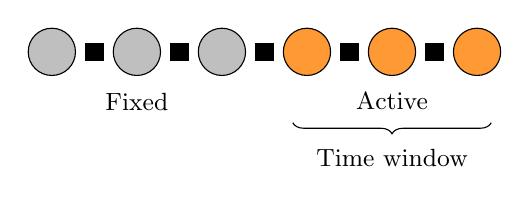
\begin{tikzpicture}[scale=0.9]
    \tikzstyle{fixed} = [circle, draw, fill=gray!50, minimum size=0.6cm, font=\small]
    \tikzstyle{active} = [circle, draw, fill=orange!80, minimum size=0.6cm, font=\small]
    \node[fixed] (x0) at (0,0) {};
    \node[fixed] (x1) at (1.2,0) {};
    \node[fixed] (x2) at (2.4,0) {};
    \node[active] (x3) at (3.6,0) {};
    \node[active] (x4) at (4.8,0) {};
    \node[active] (x5) at (6,0) {};
    \node[factor] at (0.6,0) {}; \node[factor] at (1.8,0) {}; \node[factor] at (3,0) {};
    \node[factor] at (4.2,0) {}; \node[factor] at (5.4,0) {};
    \node[font=\small] at (1.2,-0.7) {Fixed};
    \node[font=\small] at (4.8,-0.7) {Active};
    \draw[decorate,decoration={brace,amplitude=4pt,mirror}] (3.4,-1) -- (6.2,-1);
    \node[font=\small] at (4.8,-1.5) {Time window};
\end{tikzpicture}
\caption{Vertex fixing: gray = fixed (not optimized), orange = active (optimized).}
\end{figure}

\subsubsection*{3b.i Performance Analysis [9 marks]}

Figures~\ref{fig:q3b_chi2} and \ref{fig:q3b_timing} show the $\chi^2$ and optimization time comparison.

\begin{figure}[H]
\centering
\includegraphics[width=0.85\textwidth]{q3_b10.png}
\caption{Q3b: $\chi^2$ comparison. Original G2O (blue) and fixed G2O (orange) grow similarly. After unfixing and final optimization, both converge to comparable values.}
\label{fig:q3b_chi2}
\end{figure}

\begin{figure}[H]
\centering
\includegraphics[width=0.85\textwidth]{q3_b11.png}
\caption{Q3b: Optimization time. Fixed G2O (red) remains near zero during the run, while original G2O (green) increases steadily. Both spike at the end when all vertices are unfixed and a final optimization is performed.}
\label{fig:q3b_timing}
\end{figure}

\textbf{Key observations:}
\begin{itemize}
\item The fixed G2O achieves near-constant optimization time during the run because the effective number of free variables is bounded by the time window size.
\item The original G2O's optimization time grows as the full graph expands.
\item The $\chi^2$ values are similar because both systems have the same edges; fixing does not remove edges, only freezes vertex values.
\item At the very end, all vertices are unfixed and a final optimization is run, causing a large spike in computation time for both systems.
\end{itemize}

\textbf{Reason:} Fixed vertices are excluded from the Hessian computation, reducing the effective optimization dimension from the full trajectory length to just the time window.

\subsubsection*{3b.ii Covariance Behavior [6 marks]}

Figure~\ref{fig:q3b_cov} shows the error plots for the fixed G2O system. The covariance behavior is markedly different from the standard G2O system (Figure~\ref{fig:q3b_g2o_errors}).

\begin{figure}[H]
\centering
\begin{subfigure}[b]{\textwidth}
    \centering
    \includegraphics[width=0.85\textwidth]{q3_b1.png}
    \caption{Original G2O $x$ error---within bounds throughout}
\end{subfigure}
\vspace{0.2em}
\begin{subfigure}[b]{\textwidth}
    \centering
    \includegraphics[width=0.85\textwidth]{q3_b5.png}
    \caption{Original G2O $y$ error---within bounds throughout}
\end{subfigure}
\caption{Q3b: Original G2O error plots. Errors remain within $\pm 2\sigma$ bounds. Consistent.}
\label{fig:q3b_g2o_errors}
\end{figure}

\begin{figure}[H]
\centering
\begin{subfigure}[b]{\textwidth}
    \centering
    \includegraphics[width=0.85\textwidth]{q3_b4.png}
    \caption{Fixed G2O $x$ error---error exceeds narrow bounds during run, recovers after unfixing ($t \approx 100$\,s)}
\end{subfigure}
\vspace{0.2em}
\begin{subfigure}[b]{\textwidth}
    \centering
    \includegraphics[width=0.85\textwidth]{q3_b8.png}
    \caption{Fixed G2O $y$ error---similar pattern of underestimated covariance during run}
\end{subfigure}
\caption{Q3b: Fixed G2O error plots. During the run, the $\pm 2\sigma$ bounds are artificially narrow ($\sim\!\pm 0.5$\,m) due to fixing. After all vertices are unfixed ($t \approx 100$\,s), bounds expand and errors return within them.}
\label{fig:q3b_cov}
\end{figure}

\textbf{During the run:}
\begin{itemize}
\item The $\pm 2\sigma$ bounds are artificially narrow (e.g., $\pm 0.5$\,m for $x$) while the actual error reaches $\pm 2$\,m
\item This is because fixed vertices are treated as perfectly known, breaking the correlation chains through the trajectory and suppressing uncertainty propagation
\end{itemize}

\textbf{After unfixing (at $t \approx 100$\,s):}
\begin{itemize}
\item All vertices are unfixed and a final optimization runs
\item The covariance bounds suddenly expand as the full uncertainty propagates through the now-free graph
\item The errors return within the corrected $\pm 2\sigma$ bounds
\end{itemize}

\textbf{Cause:} Fixing a vertex is equivalent to conditioning on its value---it assumes zero uncertainty for that state. This eliminates the contribution of fixed vertices to the marginal covariance, causing systematic underestimation.

\subsubsection*{3b.iii Strategy Evaluation [4 marks]}

\textbf{Assessment: Moderately successful, with caveats.}

\textbf{During the run:}
\begin{itemize}
\item The strategy achieves near-constant optimization time, making it suitable for real-time operation
\item However, the covariance estimates are unreliable---the system appears overconfident, which could lead to poor decisions if uncertainty estimates are used for planning or data association
\end{itemize}

\textbf{After the final optimization:}
\begin{itemize}
\item Full accuracy and correct covariance estimates are recovered once all vertices are unfixed
\item The final optimization is computationally expensive (comparable to the original system)
\end{itemize}

\textbf{Conclusion:} This strategy is well-suited for scenarios where real-time operation is needed during data collection, with accurate results computed offline afterwards. It is not suitable for applications requiring reliable uncertainty estimates during operation, such as active exploration or safety-critical navigation.

%==============================================================================
\appendix
\section{Jacobian Derivations}

\textbf{Process Model Edge:} For error $\mathbf{e} = \mathbf{M}^{-1}(\mathbf{x}_{k+1} - \mathbf{x}_k) - \mathbf{z}$:
\begin{align}
\mathbf{J}_2 &= \frac{\partial\mathbf{e}}{\partial\mathbf{x}_{k+1}} = \mathbf{M}^{-1} = \frac{1}{\Delta T}\begin{bmatrix} \cos\theta & \sin\theta & 0 \\ -\sin\theta & \cos\theta & 0 \\ 0 & 0 & 1 \end{bmatrix} \\
\mathbf{J}_1 &= \frac{\partial\mathbf{e}}{\partial\mathbf{x}_k} = \frac{1}{\Delta T}\begin{bmatrix} -\cos\theta & -\sin\theta & -\sin\theta\Delta x + \cos\theta\Delta y \\ \sin\theta & -\cos\theta & -\cos\theta\Delta x - \sin\theta\Delta y \\ 0 & 0 & -1 \end{bmatrix}
\end{align}

\textbf{Range-Bearing Edge:} For $\mathbf{h} = [r, \beta]^T$ with $dx = l_x - p_x$, $dy = l_y - p_y$:
\begin{align}
\frac{\partial\mathbf{h}}{\partial\mathbf{x}} &= \begin{bmatrix} -dx/r & -dy/r & 0 \\ dy/r^2 & -dx/r^2 & -1 \end{bmatrix}, \quad
\frac{\partial\mathbf{h}}{\partial\mathbf{m}} = \begin{bmatrix} dx/r & dy/r \\ -dy/r^2 & dx/r^2 \end{bmatrix}
\end{align}

\end{document}
